\begin{figure}
    \centering
    \footnotesize
    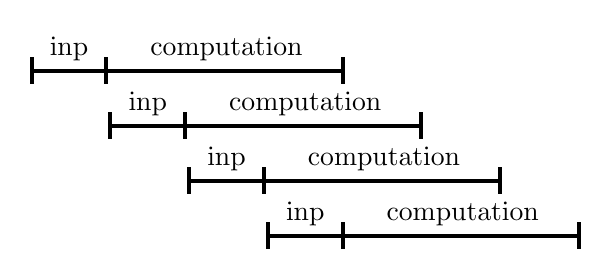
\begin{tikzpicture}
    \foreach \x in {0, 1, 2,...,3} {
        \draw[|-|, black, line width=0.5mm] (\x,-\x*0.7) to (\x+1,-\x*0.7);
        \path (\x,-\x*0.7) -- (\x+1,-\x*0.7) node [midway, above] {inp};
        \draw[-|, black, line width=0.5mm, shorten <=-0.1mm] (\x+1,-\x*0.7) to (\x+4,-\x*0.7);
        \path (\x+1,-\x*0.7) -- (\x+4,-\x*0.7) node [midway, above] {computation};
    }
    \end{tikzpicture}
    \caption{Parallelized beacon protocol, with offset input collection and overlapping computation.}\label{fig:beacon_parallel_timeline}
\end{figure}

\begin{figure}
    \centering
    \footnotesize
    \begin{tikzpicture}[xscale=0.95,
        comp line/.style={-o, GoogleIndigo, line width=0.5mm, shorten <=-0.1mm},
        incomplete comp line/.style={comp line, -ss},
        input line/.style={latex reversed-, dotted, black, line width=0.2mm},
    ]
    \pgfdeclarelayer{background}
    \pgfsetlayers{background,main}
    \draw[|-ss, line width=0.5mm, black] (0,0.7) to (8.5,0.7);
    \path (0,0.7) -- (8,0.7) node [midway, above] {Input Collection Stream};

    \foreach \x in {0, 1, 2} {
        \begin{pgfonlayer}{background}
            \draw[input line] (\x+1,0.7) to (\x+1,-\x*0.7);
        \end{pgfonlayer}
        \draw[comp line] (\x+1,-\x*0.7) to (\x+4,-\x*0.7);
        \path (\x+1,-\x*0.7) -- (\x+4,-\x*0.7) node [midway, above] {\contour{white}{Computation}};
    }
    \foreach \x in {3, 4} {
        \begin{pgfonlayer}{background}
        \draw[input line] (\x+1,0.7) to (\x+1,{-(\x-3)*0.7});
        \end{pgfonlayer}
        \draw[comp line] (\x+1,{-(\x-3)*0.7}) to (\x+4,{-(\x-3)*0.7});
        \path (\x+1,{-(\x-3)*0.7}) -- (\x+4,{-(\x-3)*0.7}) node [midway, above] {\contour{white}{Computation}};
    }

    \begin{pgfonlayer}{background}
    \draw[input line] (6,0.7) to (6,-0.7*2);
    \end{pgfonlayer}
    \draw[incomplete comp line] (6,-0.7*2) to (8.5,-0.7*2);
    \path (6+1.5,-0.7*2) node [above] {\contour{white}{Computation}};

    \begin{pgfonlayer}{background}
    \draw[input line] (7,0.7) to (7,0);
    \end{pgfonlayer}
    \draw[incomplete comp line] (7,0) to (8.5,0);

    \begin{pgfonlayer}{background}
    \draw[input line] (8,0.7) to (8,-0.7);
    \end{pgfonlayer}
    \draw[incomplete comp line] (8,-0.7) to (8.5,-0.7);

    \end{tikzpicture}
    \caption{Parallelized beacon protocol, with input collection stream and overlapping computation. A circle denotes outputting at the end of the computation.}\label{fig:beacon_parallel_timeline_real}
\end{figure}

